\documentclass[tikz, border=14pt]{standalone}
\usepackage{amsmath, amssymb}
\usetikzlibrary{arrows.meta, fit, backgrounds, calc}

\pgfdeclarelayer{shadows}
\pgfsetlayers{background,shadows,main}

%% ── Palette ──────────────────────────────────────────────────────────────────
\definecolor{cin}{RGB}{41,128,185}
\definecolor{cenc}{RGB}{142,68,173}
\definecolor{cgnn}{RGB}{39,174,96}
\definecolor{cagg}{RGB}{230,126,34}
\definecolor{cpol}{RGB}{192,57,43}
\definecolor{cout}{RGB}{52,73,94}

\tikzset{
  %% Content box
  B/.style 2 args={draw=#1, fill=#1!10, rounded corners=4pt,
    align=center, font=\small, inner sep=5pt, text width=#2},
  %% Arrow (with head, rounded bends)
  A/.style={-{Stealth[length=3.5pt,width=3pt]}, line width=0.75pt,
            color=gray!60, rounded corners=4pt},
  %% Plain line (no head, rounded bends) – used before junctions
  L/.style={line width=0.75pt, color=gray!60, rounded corners=4pt},
  %% Section background panel  (inner sep reduced to 6 pt for less dead-space)
  BG/.style={fill=#1!6, draw=#1!40, line width=0.8pt,
             rounded corners=7pt, inner sep=6pt},
  %% Section header chip
  HC/.style={fill=#1!80, rounded corners=3pt,
             font=\footnotesize\bfseries\color{white},
             inner xsep=7pt, inner ysep=3pt, anchor=south west}
}

%% ── Two fixed horizontal lanes ───────────────────────────────────────────────
%%   y_A = -2.5   Lane A  (node-feature path)
%%   y_B = -5.8   Lane B  (metadata path)       ← tightened from -6.0
%%   y_M = -4.15  Merge   (midpoint A↔B)        ← tightened from -4.25
%%
%%   Section boundaries verified (box inner 0.176 cm, bg inner 0.211 cm):
%%     bg1 right ≈ 1.79   bg2 left ≈ 2.01   gap 0.22 cm ✓
%%     bg2 right ≈ 9.99   bg3 left ≈ 10.21  gap 0.22 cm ✓
%%     bg3 right ≈ 14.69  bg4 left ≈ 15.01  gap 0.32 cm ✓
%%     bg4 right ≈ 23.09  bg5 left ≈ 23.51  gap 0.42 cm ✓

\begin{document}
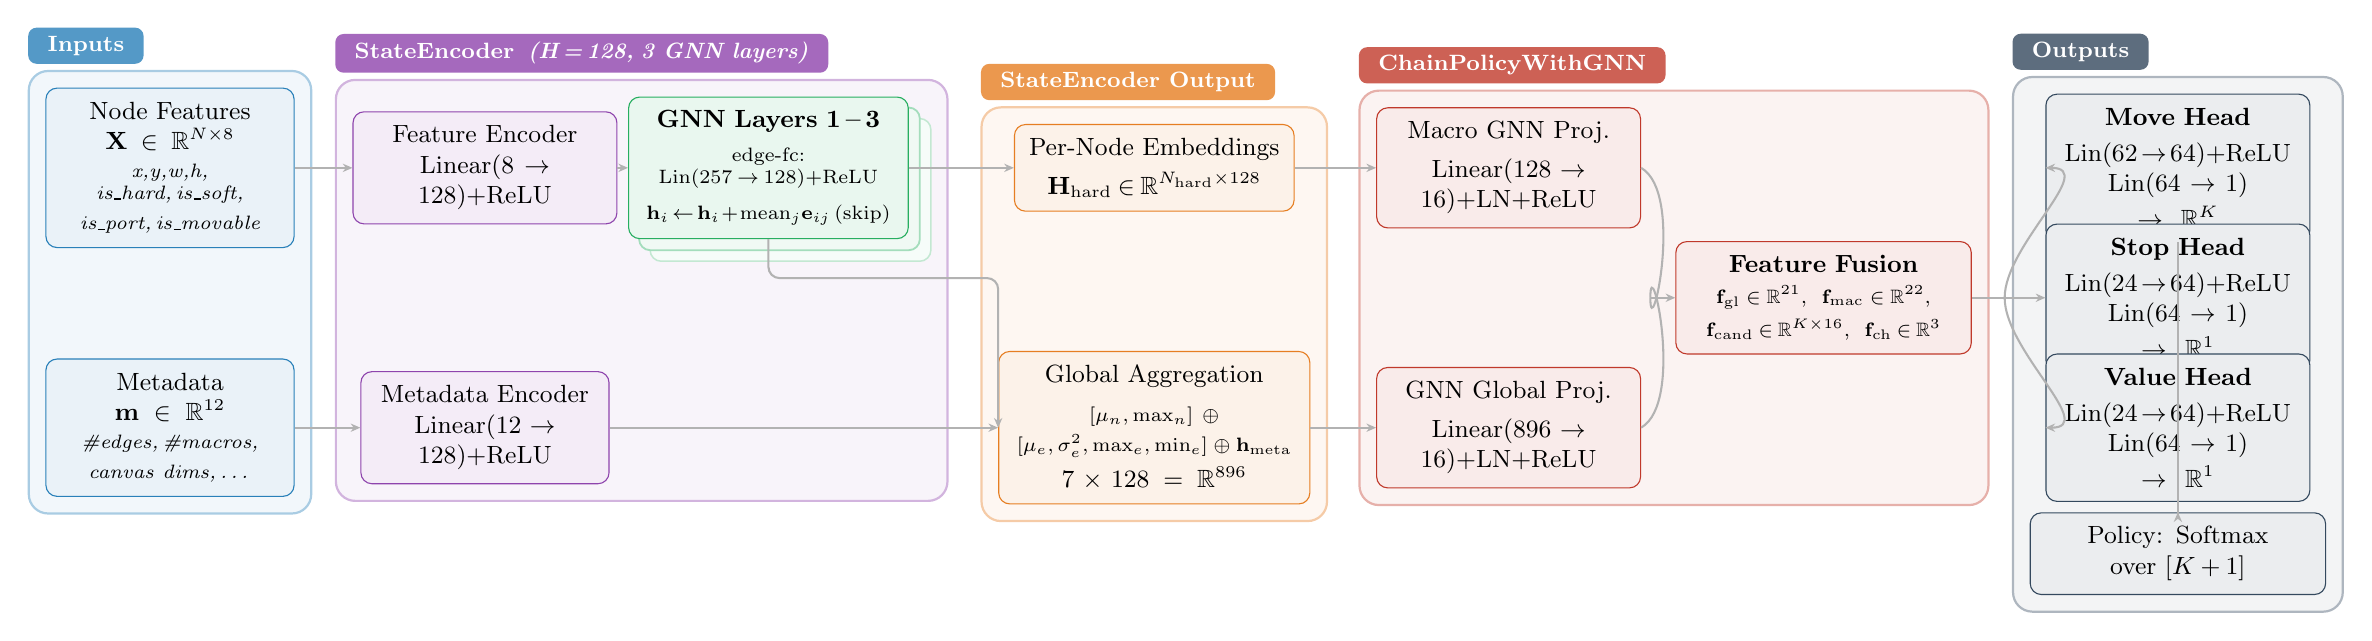
\begin{tikzpicture}[x=1cm, y=1cm]

\def\yA{-2.5}
\def\yB{-5.8}
\def\yM{-4.15}

%%════════════════════════════════════════════════════════════════════════════
%%  C1  INPUTS
%%════════════════════════════════════════════════════════════════════════════
\node[B={cin}{2.8cm}] (inp_node) at (0,\yA) {%
  Node Features \\ $\mathbf{X}\in\mathbb{R}^{N\times8}$ \\[2pt]
  {\scriptsize\itshape x,y,w,h,\\is\_hard,\,is\_soft,\\is\_port,\,is\_movable}};

\node[B={cin}{2.8cm}] (inp_meta) at (0,\yB) {%
  Metadata \\ $\mathbf{m}\in\mathbb{R}^{12}$ \\[2pt]
  {\scriptsize\itshape \#edges,\,\#macros,\\canvas dims,\,\ldots}};

%%════════════════════════════════════════════════════════════════════════════
%%  C2  STATE ENCODER
%%    Lane A:  feat_enc  →  GNN stack (3 layers, stacked-card graphic)
%%    Lane B:  meta_enc  (long bypass to C3 global)
%%════════════════════════════════════════════════════════════════════════════
\node[B={cenc}{3.0cm}] (feat_enc) at (4.0,\yA) {%
  Feature Encoder \\ Linear$(8\!\to\!128)$+ReLU};

\node[B={cenc}{2.8cm}] (meta_enc) at (4.0,\yB) {%
  Metadata Encoder \\ Linear$(12\!\to\!128)$+ReLU};

%% GNN front box (anchors used for shadow offsets)
\node[B={cgnn}{3.2cm}] (gnn) at (7.6,\yA) {%
  \textbf{\mbox{GNN Layers 1\,–\,3}}\\[4pt]
  {\scriptsize edge-fc: Lin$(257\!\to\!128)$+ReLU\\[2pt]
   $\mathbf{h}_i\!\leftarrow\!\mathbf{h}_i\!+\!\mathrm{mean}_j\mathbf{e}_{ij}$\,(skip)}};

\coordinate (gnn_ext) at ($(gnn.south east)+(0.28,-0.28)$);

\begin{pgfonlayer}{shadows}
  \fill[cgnn!4, rounded corners=4pt, draw=cgnn!28, line width=0.55pt]
    ($(gnn.south west)+(0.28,-0.28)$) rectangle ($(gnn.north east)+(0.28,-0.28)$);
  \fill[cgnn!7, rounded corners=4pt, draw=cgnn!42, line width=0.65pt]
    ($(gnn.south west)+(0.14,-0.14)$) rectangle ($(gnn.north east)+(0.14,-0.14)$);
\end{pgfonlayer}

%%════════════════════════════════════════════════════════════════════════════
%%  C3  STATE ENCODER OUTPUT
%%════════════════════════════════════════════════════════════════════════════
\node[B={cagg}{3.2cm}] (per_node) at (12.5,\yA) {%
  Per-Node Embeddings \\[3pt]
  $\mathbf{H}_\text{hard}\!\in\!\mathbb{R}^{N_\text{hard}\times128}$};

\node[B={cagg}{3.6cm}] (global) at (12.5,\yB) {%
  Global Aggregation \\[3pt]
  {\scriptsize$[\mu_n,\max_n]\oplus[\mu_e,\sigma^2_e,\max_e,\min_e]\oplus\mathbf{h}_\text{meta}$}\\[2pt]
  $7\times128=\mathbb{R}^{896}$};

%%════════════════════════════════════════════════════════════════════════════
%%  C4  CHAIN POLICY WITH GNN
%%    Projections on Lane A/B  →  Feature Fusion at Merge
%%════════════════════════════════════════════════════════════════════════════
\node[B={cpol}{3.0cm}] (mac_proj) at (17.0,\yA) {%
  Macro GNN Proj.\\[3pt] Linear$(128\!\to\!16)$+LN+ReLU};

\node[B={cpol}{3.0cm}] (gnn_proj) at (17.0,\yB) {%
  GNN Global Proj.\\[3pt] Linear$(896\!\to\!16)$+LN+ReLU};

\node[B={cpol}{3.4cm}] (fusion) at (21.0,\yM) {%
  \textbf{Feature Fusion}\\[3pt]
  {\scriptsize
    $\mathbf{f}_\text{gl}\!\in\!\mathbb{R}^{21}$,\;
    $\mathbf{f}_\text{mac}\!\in\!\mathbb{R}^{22}$,\\[1pt]
    $\mathbf{f}_\text{cand}\!\in\!\mathbb{R}^{K\times16}$,\;
    $\mathbf{f}_\text{ch}\!\in\!\mathbb{R}^3$}};

%%════════════════════════════════════════════════════════════════════════════
%%  C5  OUTPUTS  (MLP head + logit combined)
%%════════════════════════════════════════════════════════════════════════════
\node[B={cout}{3.0cm}] (move_out) at (25.5,\yA) {%
  \textbf{Move Head}\\[2pt]
  Lin$(62\!\to\!64)$+ReLU\\Lin$(64\!\to\!1)$\\[2pt]
  $\to\mathbb{R}^K$};

\node[B={cout}{3.0cm}] (stop_out) at (25.5,\yM) {%
  \textbf{Stop Head}\\[2pt]
  Lin$(24\!\to\!64)$+ReLU\\Lin$(64\!\to\!1)$\\[2pt]
  $\to\mathbb{R}^1$};

\node[B={cout}{3.0cm}] (val_out) at (25.5,\yB) {%
  \textbf{Value Head}\\[2pt]
  Lin$(24\!\to\!64)$+ReLU\\Lin$(64\!\to\!1)$\\[2pt]
  $\to\mathbb{R}^1$};

\node[B={cout}{3.4cm}] (softmax) at (25.5,-7.4) {%
  Policy: Softmax over $[K\!+\!1]$};

%%════════════════════════════════════════════════════════════════════════════
%%  ARROWS
%%════════════════════════════════════════════════════════════════════════════

%% ── Straight horizontals ──────────────────────────────────────────────────
\draw[A] (inp_node.east) -- (feat_enc.west);
\draw[A] (inp_meta.east) -- (meta_enc.west);
\draw[A] (feat_enc.east) -- (gnn.west);
\draw[A] (meta_enc.east) -- (global.west);      %% Lane-B bypass (safe: GNN is on Lane A)
\draw[A] (gnn.east)      -- (per_node.west);
\draw[A] (per_node.east) -- (mac_proj.west);
\draw[A] (global.east)   -- (gnn_proj.west);

%% ── GNN → global  (cross-lane Z-route with rounded bends) ─────────────────
\draw[A] (gnn.south) -- (7.6,-3.9)
         -- (global.west |- 0,-3.9)
         -- (global.west);

%% ── V-convergence into Fusion ─────────────────────────────────────────────
%%   Each projection arm curves smoothly to meet a shared bus point,
%%   which then feeds into fusion.west as one clean arrow.
\draw[L] (mac_proj.east) to[out=-30, in=-90] (18.8,\yM);
\draw[L] (gnn_proj.east) to[out=30,  in=90]  (18.8,\yM);
\draw[A] (18.8,\yM) -- (fusion.west);

%% ── Fan from Fusion  ──────────────────────────────────────────────────────
%%   Central bus exits fusion.east; three arms curve to their targets.
\draw[L] (fusion.east) -- (23.3,\yM);
\draw[A] (23.3,\yM) to[out=90,  in=0] (move_out.west);   %% arcs up
\draw[A] (23.3,\yM) --              (stop_out.west);      %% straight (same y)
\draw[A] (23.3,\yM) to[out=-90, in=0] (val_out.west);    %% arcs down

%% ── Move + Stop → Policy Softmax ─────────────────────────────────────────
\draw[L] (move_out.south) -- (25.5,-6.9);
\draw[L] (stop_out.south) -- (25.5,-6.9);
\draw[A] (25.5,-6.9) -- (softmax.north);

%%════════════════════════════════════════════════════════════════════════════
%%  SECTION BACKGROUNDS
%%════════════════════════════════════════════════════════════════════════════
\begin{pgfonlayer}{background}
  \node[BG=cin,  fit=(inp_node)(inp_meta)]                          (bg1){};
  \node[BG=cenc, fit=(feat_enc)(meta_enc)(gnn)(gnn_ext)]            (bg2){};
  \node[BG=cagg, fit=(per_node)(global)]                            (bg3){};
  \node[BG=cpol, fit=(mac_proj)(gnn_proj)(fusion)]                  (bg4){};
  \node[BG=cout, fit=(move_out)(stop_out)(val_out)(softmax)]        (bg5){};

  \node[HC=cin]  at ($(bg1.north west)+(0,2pt)$) {Inputs};
  \node[HC=cenc] at ($(bg2.north west)+(0,2pt)$)
    {StateEncoder\enspace\textit{(H\,=\,128,\;3 GNN layers)}};
  \node[HC=cagg] at ($(bg3.north west)+(0,2pt)$) {StateEncoder Output};
  \node[HC=cpol] at ($(bg4.north west)+(0,2pt)$) {ChainPolicyWithGNN};
  \node[HC=cout] at ($(bg5.north west)+(0,2pt)$) {Outputs};
\end{pgfonlayer}

\end{tikzpicture}
\end{document}
